\chapter{IMSI Catcher Detection}
\section{Framework and Hardware}
The following section will give a short overview of the OsmocomBB framework and how it works in conjunction with the Motorola C123 mobile phone to enable information harvesting for the \gls{icds}.
OsmocomBB is one of many \gls{osmo} projects\footnote{\url{http://osmocom.org/}} that implements the software part of a mobile phone.
Another project is OpenBSC which implements software for configuring and operating a \gls{bsc}.
OpenBSC was used to realise the Open Source IMSI Catcher \cite{dennis} and the base station that will be used later to evaluate the performance of the \gls{icds}.

\subsection{OsmocomBB}
OscmocomBB is the project that implements the baseband part of \gls{gsm} as an open source project.
Baseband means an open source software to control the baseband chip inside the mobile phone which is a different processor than the application processor.
The goal is to have, by using compatible hardware, a phone using free software only as opposed proprietary baseband implementations.
Therefor the project scope is implementing \gls{gsm} layer 1-3 as well as hardware drivers for the baseband chipset.
A simple user interface on the phone is planned but not yet implemented and a verbose user interface on the computer.
This could be beneficial to multiple areas \cite{osmo_rationale}:
\begin{itemize}
	\item \textbf{Security:} The software running on the baseband chips is highly proprietary and closed.
	The source is often disclosed only to the mobile phone manufacturers using the specific chipset.
	One cannot be sure that this software does not have bugs that could be exploited and ultimately pose a security risk to the subscriber.
	History has shown that open source projects are more secure than proprietary solutions since more people can view the source to find issues.
	If a security threat is found the bug is fixed fast and a patch is released.
	This could be a great benefit for phone users.
	\item \textbf{Education:} Currently knowledge about \gls{gsm} and its layers on a technical level is not very well spread.
	The literature so far 
	An open source implementation as a reference could serve to educate more developers generally interested in the subject of mobile communications and thus improve products and software.
	Additionally this implementation enables universities to hold practical lab courses and private persons to do hands-on experiments.
	\item \textbf{Research:} A free implementation can decouple research on \gls{gsm} technologies from the industry since key technologies are no longer only available to researchers employed to a specific company.
	Additionally this way security holes can be uncovered more easily.
	Modifications to the protocol stack can be deployed and tested in a real environment.
\end{itemize}

\subsubsection{Project Status}
At this point layer two and three do not actually run on the phone but rather on a computer to which the phone is connected via a serial cable whereas layer 1 runs inside the custom firmware on the \gls{me} itself, since the procedures on layer 1 are very time critical.
This has advantages as well as disadvantages.
The disadvantage is that in order to run an application written with OsmocomBB you always have to have a notebook in addition to the phone.
The benefit however is that during the development process, the phone does not have to be touched after an initial deployment of the firmware.
This means code can be modified, compiled and tested locally without the need of remote debugging; experimenting is considerably easier this way.
This separation however would not work in the original \gls{gsm} specification, therefore an extra interface between layer 1 and 2 had to be implemented to manage handle messages.
It is called L1CTL.

\begin{figure}
\centering
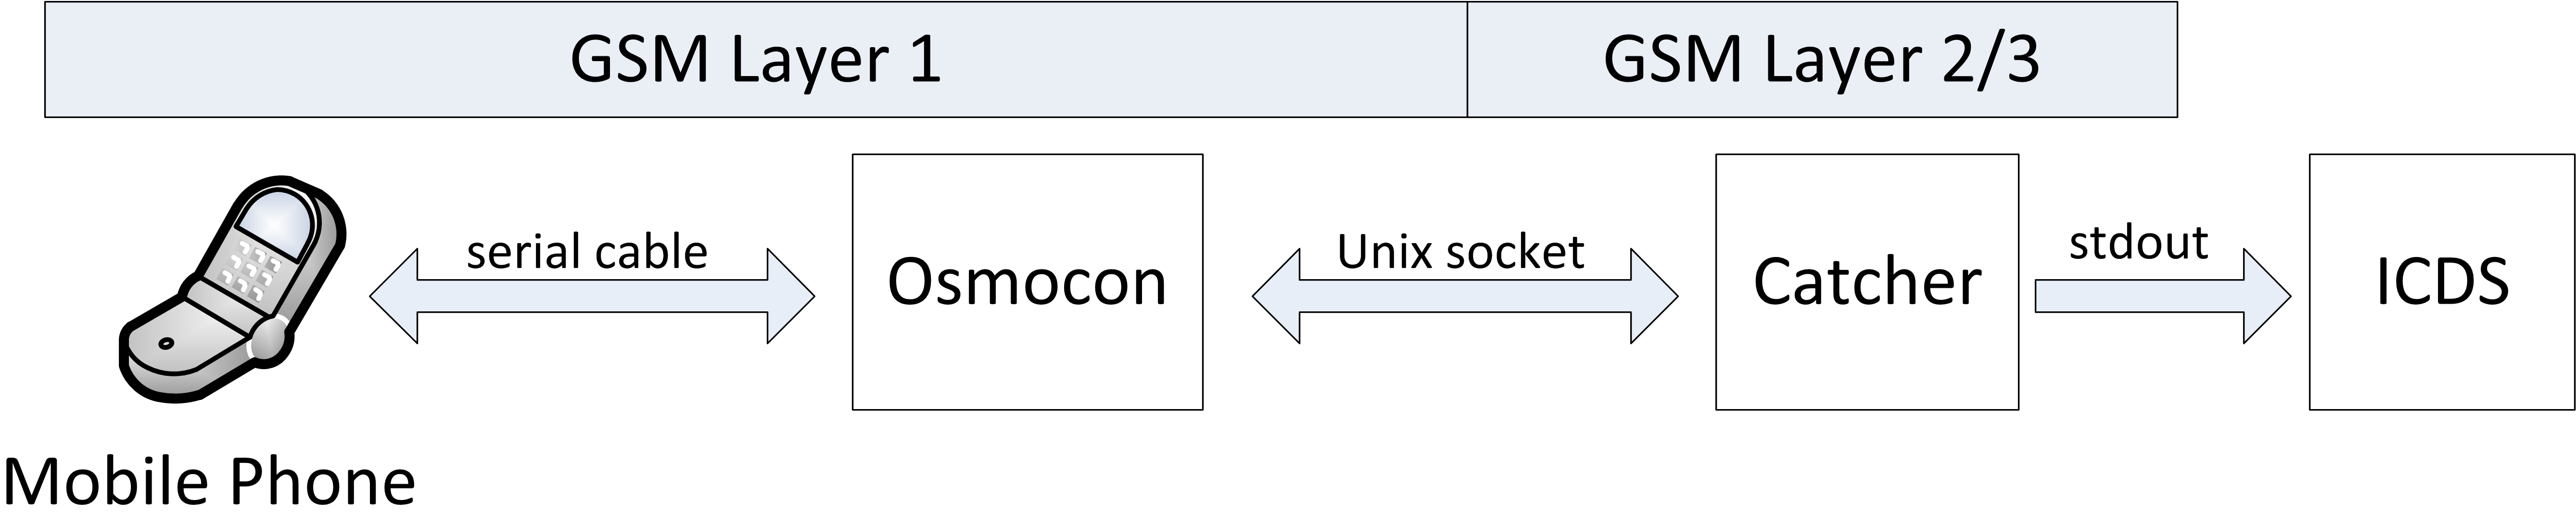
\includegraphics{../Images/OsmoStructure}
\caption{Interaction of the OsmocomBB components with the ICDS software.}
\label{fig:osmo_setup}
\end{figure}

The current state of the project is, according to a presentation given on the 27$^\text{th}$ chaos communication congress\footnote{27C3: \url{http://events.ccc.de/congress/2010/wiki/Main_Page}} by Dieter Spaar and Harald Welte, that the network layers 1-3 are fully implemented, SIM cards can be accessed or emulated and \gls{gsm} cell selection and reselection are working.
A3/A8 as well as A5/1 and A/52, Full Rate and Enhanced Full Rate codecs are there, so it is possible to do voice calls with an OsmocomBB application written for that purpose, called \texttt{mobile}.
It features a terminal/telnet based interface much like Cisco routers however there is no user interface for the phone so far or any implementation for Handovers since neighbourhood measurements are not implemented in the framework as of now.
During these calls or during the operation of other programs, it is possible to receive all the frames that are being transmitted via Wireshark from the \texttt{osmocon} application \cite{konrad}.

\subsubsection{OsmocomBB and ICDS}
The setup that is used for the \gls{icds} project can be seen in Figure \ref{fig:osmo_setup}.
It was build and tested in a Xubuntu 11.10 environment \footnote{http://xubuntu.org/} which is a more lightweight variant of the popular Debian based Ubuntu Linux distribution.
The process of acquiring, compiling and running the OsmocomBB framework itself in this environment is explained in Appendix \ref{sec:osmo_install}.
As can be seen in the diagram, layer 1 of the OsmocomBB \gls{gsm} stack runs on the phone.
It is connected via a serial cable to the computer running the \gls{icds}.
On the computer side the \texttt{osmocon} program provides a general interface to the phone.
\texttt{Osmocon} is also used to download the firmware to the Motorola C123.
Other software can communicate with \texttt{osmocon} and subsequently with the phone using unix sockets.

\texttt{Catcher} is a modified version of the \texttt{cell\_log} program by Andreas Eversberg that interfaces with \texttt{osmocon} to harvest information from \gls{bts} and forward it to the \gls{icds}.
It can be seen as a layer 3 program that scans through available frequencies and reads information from the \gls{bcch} whenever one such channel is available on the frequency at hand.
The forwarding is done directly via \texttt{stdout} since it runs as a child process of the \gls{icds}.
The functionality of \texttt{catcher} will be explained in detail in Section \ref{sec:info_gathering} while the implementation and operation of the \gls{icds} will be discussed in Section \ref{sec:icds}.

\subsection{Motorola C123}
\label{sec:osmo_phones}
Since the general idea behind OsmocomBB was to become a vendor independent open source \gls{gsm} implementation for everyone to use, there were certain requirements the targeted hardware would have to meet.
For the consumer side requirements these were having a low price and a good availability.
This criterion rules out \gls{diy} approaches since number of produced devices would be low and thus costly or a significant technical knowledge would be expected from all users to assemble the hardware.
For the developer side this would also mean implementing a lot on the lower levels of analog logic.
Therefore the Motorola C123 was chosen, an old, very cheap phone that is well spread.
It has the advantage of being very simple on the hardware side since it is based on the well documented Texas Instruments Calypso Chipset\footnote{Documentation can be found on \url{http://cryptome.org} and other sites.}
Table \ref{tab:c123_specs} shows an overview of the main specifications for the phone.
\begin{table}
\centering
	\begin{tabular}{ll}
	\toprule
	Component			&Specification\\
	\midrule
	Band 				&GSM 900, GSM 1800\\
	Size				&$101\times 45\times 21$ mm\\
	Weight				&86 g\\
	Battery				&920mAh Li-Ion battery\\
	Digital Baseband	&Texas Instruments Calypso\\
	Analog Basenand		&Texas Instruments Iota TWL3025\\
	GSM Transceiver		&Texas Instruments Rita TRF6151C\\
	\bottomrule
	\end{tabular}
	\caption{Technical specifications for the Motorola C123.}
	\label{tab:c123_specs}
\end{table}
The OsmocomBB framework should work well or with small adjustments for phones that share the same components.
Figure \ref{fig:osmo_c123} an image of the Motorola C123 circuit board with the components mentioned before.
\begin{figure}
\centering
	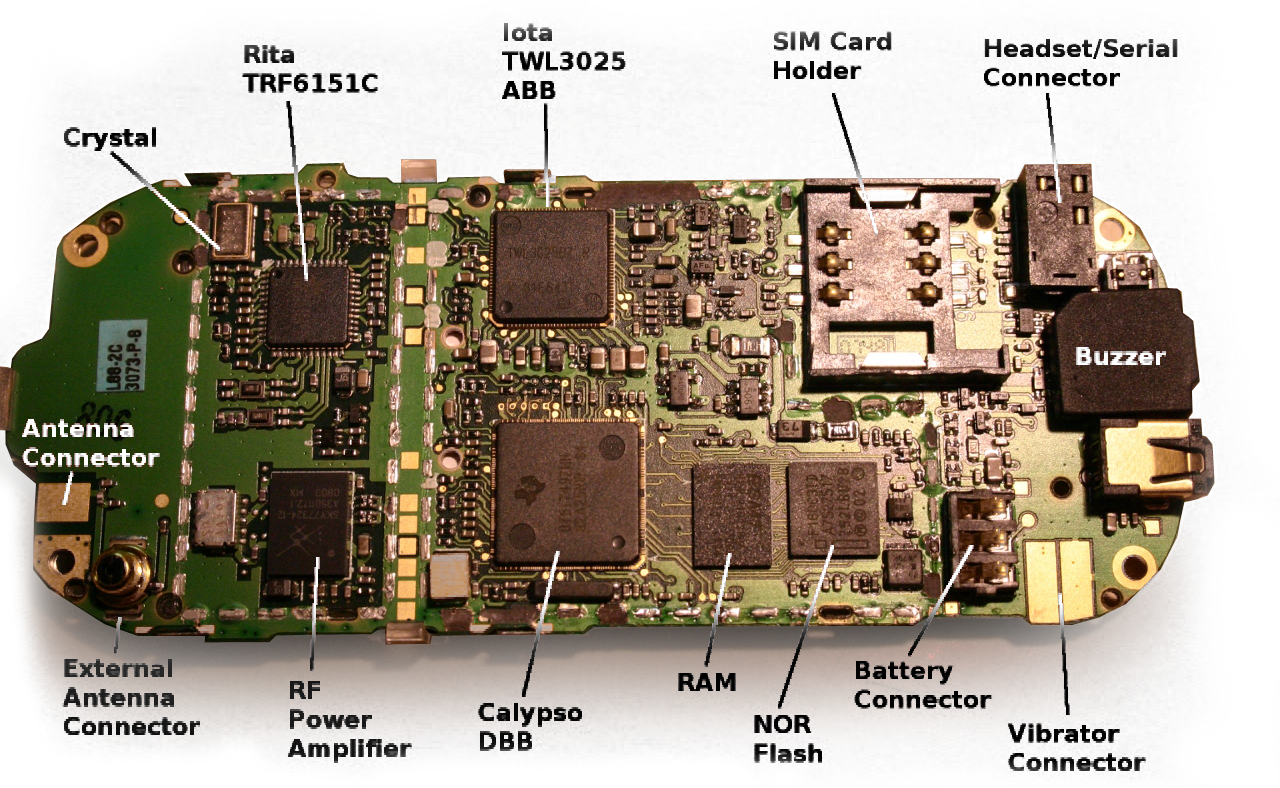
\includegraphics[width=.9\textwidth]{../Images/c123_pcb}
	\caption{Circuit board of the Motorola C123 with its components \cite{osmo_wiki_c123}.}
	\label{fig:osmo_c123}
\end{figure}
Another reason for choosing this hardware platform was that during the start of the OsmocomBB project an open source implementation of \gls{gsm} layer 1 was already available on sourceforge (TSM30 Project) that could be used as a reference.

In order to use the Motorola C123 in combination with the OsmocomBB framework the custom firmware implementing layer 1 and L1CTL has to be flashed.
This has to be done using a RS332 serial cable that is connected to the 2.5 mm audio jack.
The audio jack of the Motorola C123 and other Calypso based mobile phones typically have a 3.3 V serial port on their audio jacks.
These cables are normally referred to as T191 unlock cables 
A variety of stores around the internet sell the cables ready made for about \$10\footnote{\url{http://fonefunshop.co.uk}}.
One must be careful when using the PC's serial port to communicate with the phone though.
Since the phone's serial operates at 3.3 V and is internally connected to the 2.8 V IO-pins of the baseband processor, directly connecting it to the computers 12 V serial port will destroy the hardware.
Therefore it is recommended to use a USB serial cable.
Schematics for such an unlock cable, along with a few instructions on how to build one are given in Appendix \ref{sec:osmo_serial_schematics}.
Another issue is virtualisation.
The bootloader and the firmware can fail to be deployed correctly if a virtual machine is used as development system.
This is because the protocol used by Motorola to do the actual flashing process is \emph{very} time critical and thus timeouts can occur that are caused by the overhead the virtual machine imposes on the hardware/software communication.

\section{Procedure}
The main goal of the \gls{icds} is to reach a conclusion on whether it is safe to initiate a phone call or not, in other words if we trust all surrounding base stations.
As mentioned before as soon as a subscriber connects to an IMSI Catcher it automatically gives up information on his/her location.
Therefore this project will use a passive approach on information harvesting, meaning we will only use information that is broadcasted or freely available as to not give up any hints of the \gls{icds} being active.

To that end a four-step process is taken.
First the information is gathered.
This process is explained in detail in Section \ref{sec:info_gathering}.
After information on the surrounding \gls{bts} is ready in the \gls{icds} a set of checks is evaluated on each base station individually each yielding a specific result for the station.
These checks are called rules and discussed further along with the next two steps in Section \ref{sec:info_evaluation}.
The next step is to aggregate all the results the rules yielded for each base station into one single result for each \gls{bts}.
At last, after every \gls{bts} has its evaluation it can be decided whether to tell the subscriber it is safe to initiate a phone call or not.

\subsection{Information Gathering}
\label{sec:info_gathering}
As explained in Section \ref{sec:common_channels} every base station has an associated \gls{bcch} where information about the station and its network is spread.
\gls{bcch} frames are always sent inside a 51-Multiframe.
After the \gls{ms} has synchronised using the values on the \gls{fcch} and \gls{sch} it can determine which kind of information is hosted inside the \gls{bcch} message.
These so called System Information Messages originate at the \gls{bsc} and are produced for each \gls{bts} individually and then periodically broadcasted.
Since all the required information would not fit inside a single frame there are different kinds of System Information Messages that are distinguished by their \gls{tc} and host different kinds of information.
The type can be extracted using the \gls{fn} of the frame the message is sent in \cite{GSM2009}:
\[\text{TC}=(\text{FN} \text{ div } 51)\text{ mod } 8\]
Table \ref{tab:tc_mapping} shows how the \glspl{tc} can be mapped on those types.
\begin{table}
\centering
\begin{tabular}{lc}
\toprule
TC		&System Information Type\\
\midrule
0		&Type 1\\
1		&Type 2\\
2,6		&Type 3\\
3,7		&Type 4\\
4,5		&Any (optional)\\
\bottomrule
\end{tabular}
\caption{Type Codes and the corresponding System Information Types \cite{GSM2009}.}
\label{tab:tc_mapping}
\end{table}
For this project the System Information Type 1-4 are of interest because these are available to all \gls{ms} that tune in to the particular \gls{bcch} of the respective \gls{bts} without actively connecting to it.

The harvesting of information contained in these System Information Messages is done via the \texttt{catcher} program.
\texttt{Catcher} is implemented inside the OsmocomBB framework and connects over the \texttt{osmocon} application to the Motorola C123.
At first a sweep scan is done over all the \glspl{arfcn} to measure their reception levels in order to determine where base stations and thus \glspl{bcch} are located.
Afterwards \texttt{catcher} tunes the phone to those specific frequencies where a \gls{bts} was found 
%TODO: see whether all parameters can be harvested inside OsmocomBB
At each such frequency it waits until all the System Information Messages are gathered and extracts parameters where possible.
The parameters along with the raw data are forwarded to the main \gls{icds} application for further parsing and evaluation.
An example for a parsed System Information Type 2 Message can be seen in Figure \ref{fig:sysinfo2}.
Examples for all the System Information Messages used are located in Appendix \ref{sec:system_infos}.
\begin{figure}
\centering
\caption{System Information 2 Message with annotations \cite{protocols1999}.}
\label{fig:sysinfo2}
\end{figure}
As long as scanning mode is active all the available stations are scanned repeatedly and changes in the \gls{bts} will continuously update the data model inside the \gls{icds} software.
The parameters harvested are:
%TODO: add more detail of format
\begin{itemize}
	\item Country: The interpreted country code the base station is broadcasting.
	\item Provider: The interpreted provider code the base station is broadcasting.
	\item ARFCN: The \gls{arfcn} on which the base station is located.
	\item rxlev: Receiving strength in db.
	This parameter is measured by the Motorola C123 and not part of the System Information Messages.
	Even small changes in the location can have a large impact on this parameter due to shadowing and reflection.
	How ever it can be used in certain cases as will be discussed in Section \ref{sec:fake_parameters}.
	\item BSIC: Because of frequency reuse in a cellular network it is possible that two different base stations can sent at the same \gls{arfcn}.
	In order for the \gls{ms} to keep these apart the \gls{bsic} is also broadcasted.
	It consists of a \gls{ncc} identifying the provider, so the \gls{ms} can filter out messages that is does not need and the \gls{bcc} that must be unique for a given provider over all base station in a large area.
	\item LAC: This is the last part of the \gls{lai} (that consists of \gls{mcc} + \gls{mnc} + \gls{lac}) and is a hierarchical identifier for a given base station.
	The hierarchy is provider wide, meaning two different providers may use \glspl{lac} with a completely different numbering system.
	\item Cell ID: The Cell ID is a globally unique identifier for the cell the \gls{ms} is connected to.
	\item Neighbouring Cells: Each base station keeps a list of other base stations in the perimeter  for the \gls{ms} to scan and determine if there is a \gls{bts} with a better reception in the area.
	\item Encryption: The encryption algorithm used to encrypt the voice data.
	Note that encryption cannot actually be read passively from a base station since the encryption algorithm is determined when a connection is established.
	%TODO: find out exactly how this is done
	To not become active and connect to the station, this is harvested by tuning in to something and capture the packages that set the encryption for another mobile subscriber.
\end{itemize}
Since the \texttt{catcher} program is spawned inside the \gls{icds} application as a subprocess, information forwarding is done via stdout so new parameters could be implemented with minimal overhead.

\subsection{Information Evaluation}
\label{sec:info_evaluation}
Each base station is evaluated the moment the data completely arrived at the \gls{icds} application.
Additionally when a new \gls{bts} has been found and added all formerly discovered station are also re-evaluated since new discoveries can have an impact on the rules that evaluate the context surrounding an old base station.

As mentioned above, evaluation is done based on constructs called rules.
Each rule represents one check that can be performed on a base station and yields a result based on its findings.
Possible results are:
\begin{itemize}
	\item Critical: This means that the base station evaluated has a critical configuration error or critical settings that are not found on normal base stations, \eg unknown provider names or encryption is turned off.
	This station should not be trusted.
	\item Warning: The \gls{bts} at hand has some concerning features but it could not be said whether this really is a hint to a catcher or sheer coincidence.
	An example would be a base station having a  neighbouring cell list of which none of the cells therein have actually be found up to that point.
	The list could either be a fake or it could simply be coincidence that scan has not found any up to that point.
	\item Ok: The result is as expected.
	\item Ignore: In some cases the rule cannot yield a finding.
	In that case the state is explicitly to 'ignore' so the evaluator knows that this rule should have no influence on the final outcome.
	This is the case for example when trying to find whether the base station uses encryption or not and no other subscriber connects until a set timeout is reached.
\end{itemize}
Rules can be divided into two categories depending on what they do.
The first category are 'Configuration Rules' while the second are 'Context Rules'.
An overview as well as details on the rules implemented for each category can be found in the next two sections.

\subsubsection{Configuration Rules}
This set of rules targets the base station itself.
Rules in this category are meant to check the parameters that concern the \gls{bts} and check them for integrity and configuration mistakes that could have been made by an IMSI catcher operator.


\subsubsection{Contextual Rules}

\subsubsection{Rule Evaluation}

\subsection{Fake Parameters}
\label{sec:fake_parameters}


\section{IMSI Catcher Detection System}
\label{sec:icds}
\subsection{Implemetation}
\subsubsection{Architecture}
\subsubsection{Extensions}
\subsection{Configuration}
\subsection{Operation}
\label{sec:icds_operation}